\section{Architecture d'un système automatisé}
\label{sec:architecture}
\subsection{Architecture matérielle}
\label{subsec:architecture_materielle}
\paragraph{Un système automatisé centralisé} consiste en une unique unité centrale qui gère l'ensemble des entrées et des sorties. Cette unité centrale est donc reliée à l'ensemble des capteurs et des actionneurs.
Dans le domaine qui nous intéresse, l'unité centrale est un automate programmable industriel (API) et pourrait gérer une série d'étapes d'une chaîne de production.

\begin{minipage}{0.45\linewidth}
    \paragraph{Avantages}
    \begin{itemize}
        \item Un automate unique.
        \item Architecture de données simple.
    \end{itemize}
\end{minipage}%
%
\begin{minipage}{0.45\linewidth}
    \paragraph{Inconvénients}
    \begin{itemize}
        \item Nombre d'entrées/sorties important.
        \item Traitement d'automatisation complexe.
        \item Maintenance et évolutions difficiles.
    \end{itemize}
\end{minipage}

\lstDeleteShortInline~
\begin{UPSTIactivite}[][Architecture centralisée]
    \UPSTIquestion{Représenter l'architecture d'un système automatisé centralisé.}
    \vspace{4cm}
\end{UPSTIactivite}


\paragraph{Un système automatisé modulaire et réparti} consiste, à l'inverse, en plusieurs unités centrales qui gèrent chacune une partie de la chaine et donc des entrées et des sorties. Chaque unité centrale est reliée à un ensemble de capteurs et d'actionneurs. Un protocole de communication est mis en place entre les unités centrales.

\begin{minipage}{0.45\linewidth}
    \paragraph{Avantages}
    \begin{itemize}
        \item Nombre d'entrées/sorties limité par unité centrale.
        \item Maintenance et évolutions propres à chaque unité.
    \end{itemize}
\end{minipage}%
\hfill%
\begin{minipage}{0.5\linewidth}
    \paragraph{Inconvénients}
    \begin{itemize}
        \item Architecture de données complexe.
              \begin{itemize}
                  \item Orientation des données.
                  \item Perte de la sémantique des données qu'il faut reconstruire (union, chevauchement, \dots).
              \end{itemize}
        \item Protocole de communication à mettre en place.
    \end{itemize}
\end{minipage}

\begin{UPSTIactivite}[][Architecture modulaire]
    \UPSTIquestion{Représenter l'architecture d'un système automatisé modulaire.}
    \vspace{4cm}
\end{UPSTIactivite}
\lstMakeShortInline~


\paragraph{Critères de choix}
Le choix entre une architecture centralisée ou modulaire ainsi que les matériels et logiciels à utiliser se feront en fonction de différents critères :

\begin{minipage}{0.6\linewidth}
    \begin{itemize}
        \item Nombre d'entrées/sorties TOR.
        \item Nombre d'entrées/sorties analogiques.
        \item Communications à mettre en place entre les unités centrales (protocoles, nombres).
        \item Maintenance et évolution.
        \item Interconnexion avec le Cloud (4.0).
        \item Puissance de calcul nécessaire.
        \item Boucle de régulation intégrée ou non.
        \item Coût (matériel, chaîne de développement, \dots).
        \item Langages IEC 61131-3 supportés.
        \item Les extensions de ces langages pouvant conduire à une programmation orientée objet.
    \end{itemize}
\end{minipage}


Aussi, le choix de l'environnement de développement (IDE) est important. Il doit permettre de programmer l'ensemble des unités centrales et de gérer les communications entre elles. Il doit aussi permettre de gérer les entrées/sorties et les communications avec les capteurs/actionneurs. Ainsi, sur une architecture complexe, on fera le choix d'un IDE permettant la programmation, dans un même projet, de matériels non homogènes (d'automates de marques et/ou modèles différents).


%%% TODO: Réorganiser cette partie %%%
%%% TODO: Ajouter une figure architecture modulaire avec bus %%%

\subsection{Le système d'exploitation}
L'automate industriel programmable embarque un système d'exploitation temps réel. Ce système d'exploitation est un logiciel qui permet de gérer les ressources matérielles de l'automate (processeur, mémoire, entrées/sorties, \dots) et de fournir des services aux applications (gestion des tâches, gestion des communications, \dots).

Pour programmer efficacement et correctement un automate, il est nécessaire de comprendre, au moins sommairement, le fonctionnement du système d'exploitation.

\subsubsection{Rappels : Le cycle automate}
Un Automate Programmable Industriel (API) fonction en suivant un cycle périodique, appelé cycle automate dont la période est généralement comprise entre \SI{1}{\milli\second} et \SI{100}{\milli\second}. 
Ce cycle est composé de 4 phases répétées en boucle :

\begin{minipage}[c]{.65\linewidth}
\begin{enumerate}
    \item Traitement interne 
    \begin{itemize}
        \item Mise à jour des bits système 
        \item Requêtes en provenance de la console
        \item horodatage
        \item \dots
    \end{itemize}
    \item Lecture des entrées
    \begin{itemize}
        \item Le système met à jour l'état des entrées TOR et analogiques.
        \item \textbf{Attention : l'état des entrées ne sera pas lu en dehors de cette étape}
    \end{itemize}
    \item Traitement des programmes
    \begin{itemize}
        \item Exécution des programmes utilisateur.
        \item Exécution des programmes système.
    \end{itemize}
    \item Ecriture des sorties 
    \begin{itemize}
        \item Le système met à jour l'état des sorties TOR et analogiques.
        \item \textbf{Attention : c'est donc uniquement l'état de la sortie après exécution de tous les programmes qui sera écrit sur les sorties.}
    \end{itemize}

\end{enumerate}
\end{minipage}%
\begin{minipage}[c]{.3\linewidth}
    \begin{center}
        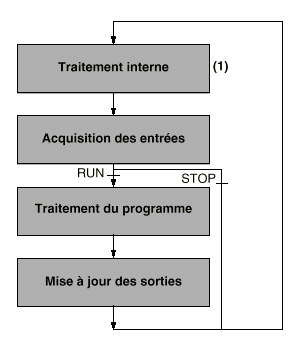
\includegraphics[width=\linewidth]{automate_cycle.png}
    \end{center}
\end{minipage}

\UPSTIinfo[Système temps réel]{
    Un système d'exploitation temps réel garantit un temps de réponse maximum à toute requête ou événement matériel.

    Ce type de système d'exploitation est utilisé dans les systèmes embarqués, les automates programmables, les systèmes de contrôle-commande, \dots En résumé, dans tous les domaines où la réactivité à un événement externe est primordiale.
}

\subsubsection{Propriétés du système d'exploitation d'un API}
Un système d'exploitation d'un API possède les propriétés suivantes :
\begin{description}
    \item[Temps réel : ] par la mise en place d'un chien de garde (watchdog).
    \item[Interruptible : ] les tâches peuvent être interrompues par une tâche de \textbf{priorité supérieure} parce que l'événement qu'elle traite est \textbf{fugitif} ou d'\textbf{importance} pour l'application.
    \item[Mono/Multi-tâche : ] Plusieurs tâches peuvent être exécutées de façon apparemment simultanée.
    \item[Accès facilité aux entrées/sorties.]
    \item[Accès facilité à la mémoire : ] Permet de partager des données entre les tâches, de gérer les accès concurrents à la mémoire, \dots
    \item[Interaction avec le programme utilisateur].
\end{description}

Les événements sont capturés par des fonctions appelées \textbf{event handlers}. Ces fonctions sont automatiquement appelées par le système d'exploitation lorsqu'un événement défini se produit.


\UPSTIinfo[Système Multitâches]{
    Un système multitâche permet d'exécuter plusieurs tâches "en même temps". En réalité, une stratégie de priorité des tâches est mis en place. Selon le nombre de processeurs présents et le nombre de tâches, elles seront exécutées en parallèle ou en alternance.
}